\chapter{Results}
\label{chap:results}

%% PURPOSE: This chapter presents the raw findings, one section per RQ.
%% Keep it factual — save interpretation for Chapter 6 (Discussion).
%% Each section should reference the specific figure/table produced by the pipeline.

\section{Overview}
\label{sec:results-overview}
% TODO: Write a 3-5 sentence roadmap of the chapter. State the order in which
% the five RQs are addressed and give the reader one headline result per RQ
% so they know what to look for as they read.
This chapter presents the empirical results of the study, structured sequentially around the five research questions: the identification of behavioral profiles (RQ1), their temporal and cross-context robustness (RQ2), their association with final grades (RQ3), their predictive utility (RQ4), and finally the interpretability of the signals of success and risk (RQ5). The aim of this section is to report the data and metrics objectively, leaving the deeper interpretation of these findings and their connection to the methodological context for the Discussion chapter.

\section{RQ1: Identification of Choreographies}
\label{sec:rq1-results}
% TODO: Present the k-selection results:
%   - Table or figure of silhouette scores and inertia for k = 2..10
%     (k_selection.png).
%   - Justification for k = 4 based on the silhouette peak.
%
% Present the four discovered choreographies:
%   - For each cluster: name, size (student-weeks, % of total), top 6
%     over-represented features with lift values (from run_clustering.py
%     characterization output).
%   - Include the UMAP visualization (umap_clusters.png) and comment on
%     the degree of visual separation between clusters.
%
% Present the validation against ground-truth archetypes:
%   - Cluster × archetype contingency table (row %, from cluster_vs_archetype.csv).
%   - Dominant archetype and purity per cluster.
%   - ARI and NMI values and their interpretation (reference Section~\ref{sec:evaluation-design}).
The first step was to decide how many groups to create. As illustrated in Figure~\ref{fig:k-selection}, the automatic metrics did not point to a single clear value. Since the UMAP projection showed that behaviors blend somewhat rather than forming isolated islands, both four and five groups were tested. Both reached essentially the same accuracy, so the simpler, more direct option was chosen: four groups to avoid redundant profiles.

\begin{figure}[ht]\centering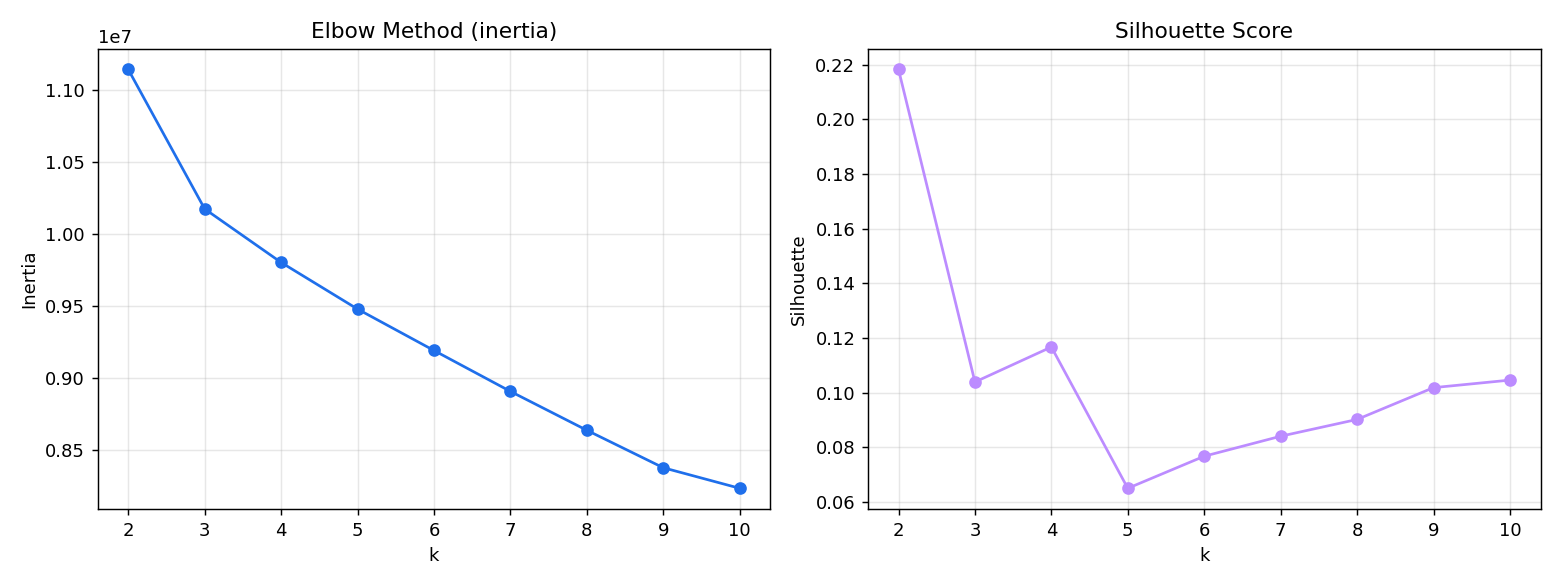
\includegraphics[width=0.8\textwidth]{figures/k_selection.png}\caption{K-selection results: silhouette scores and inertia for $k = 2..10$. The silhouette peak at $k = 4$ supports the choice of four clusters.}\label{fig:k-selection}\end{figure}

As shown in Figure~\ref{fig:umap}, clustering recovered the underlying structure with an Adjusted Rand Index of 0.532 and a Normalized Mutual Information of 0.593. These values are not perfect, but they indicate a good recovery: the model captured the main behavioral structure, while reflecting a natural overlap between students. This is visible in the purity of each group. The algorithm isolated the Balanced Engager almost perfectly (95.8\% purity) and separated the Steady Worker (63.2\%) and the Minimal Browser (56.8\%) well. The Night Crammer, however, reached only 42.6\% purity: studying late at night or early in the morning is such a dominant trait that the algorithm grouped together students who behaved differently during the rest of the day, as long as they shared this nocturnal timing.

\begin{figure}[ht]\centering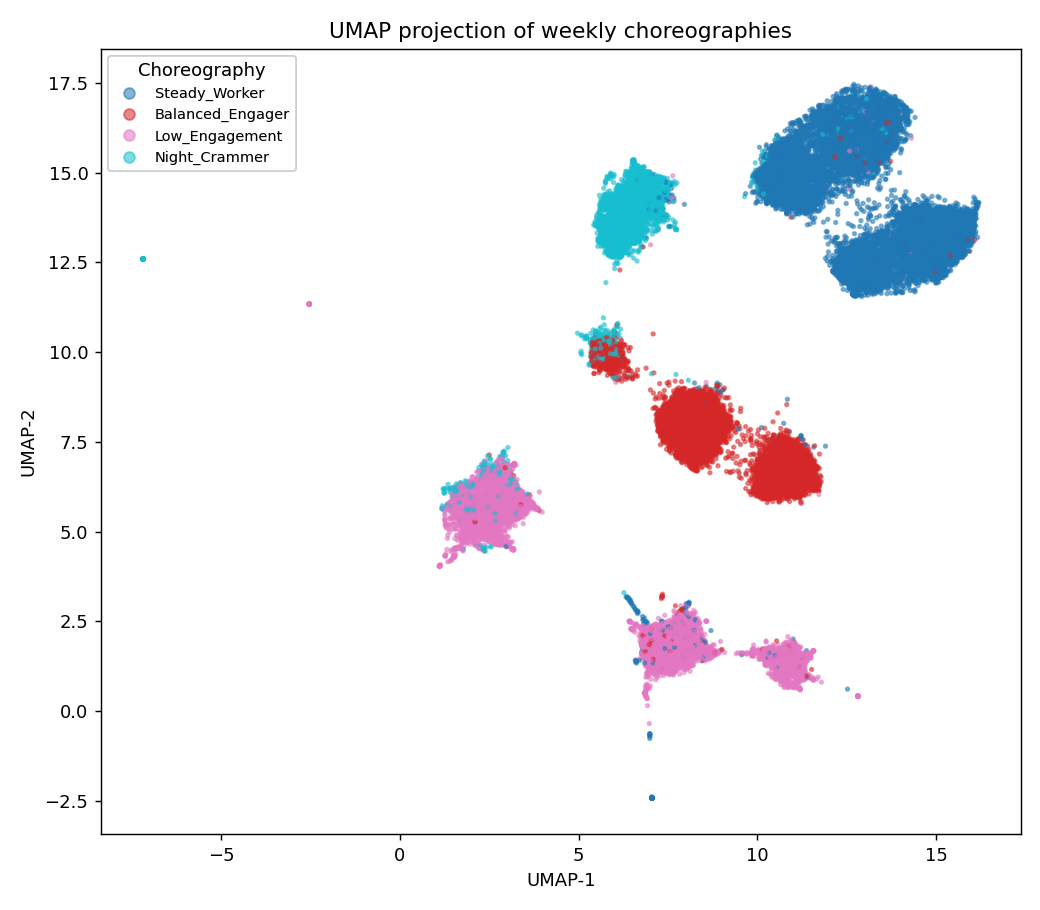
\includegraphics[width=0.55\textwidth]{figures/umap_clusters.png}\caption{UMAP projection of the four discovered choreographies.}\label{fig:umap}\end{figure}

\section{RQ2: Robustness (Temporal and Cross-Context)}
\label{sec:rq2-results}
% TODO: (a) Temporal stability:
%   - Report mean, std, min/max of the week-over-week ARI series.
%   - Report mean same-cluster retention percentage.
%   - Include temporal_ari.png (ARI + retention over the academic year).
%   - Present the transition matrix (transition_matrix.png) and report the
%     diagonal stickiness values per cluster.
%
% (b) Cross-context stability:
%   - Present the choreography share (%) table by Grade_Level.
%   - Report grade-std and state-std for each cluster.
%   - Include profile_by_grade.png and profile_by_state.png.
%   - Report cosine similarity of per-cluster behavioral signatures
%     across grade bands (K-5 vs 6-12), and the mean across all clusters.
The temporal stability analysis showed that students maintain a high degree of consistency in their learning patterns throughout the year (see Figure~\ref{fig:temporal_ari}). This translated into a week-over-week Adjusted Rand Index (ARI) of around 0.80 and a same-profile retention rate of roughly 91\%. The only marked fluctuation occurred during the winter break, where the ARI dropped to about 0.50, reflecting the disruption of routines typical of a holiday period. However, it is important to acknowledge that this exceptionally high baseline stability is partially a structural artifact of the synthetic data generation process, wherein students are simulated from a fixed underlying archetype.

\begin{figure}[H]
    \centering
    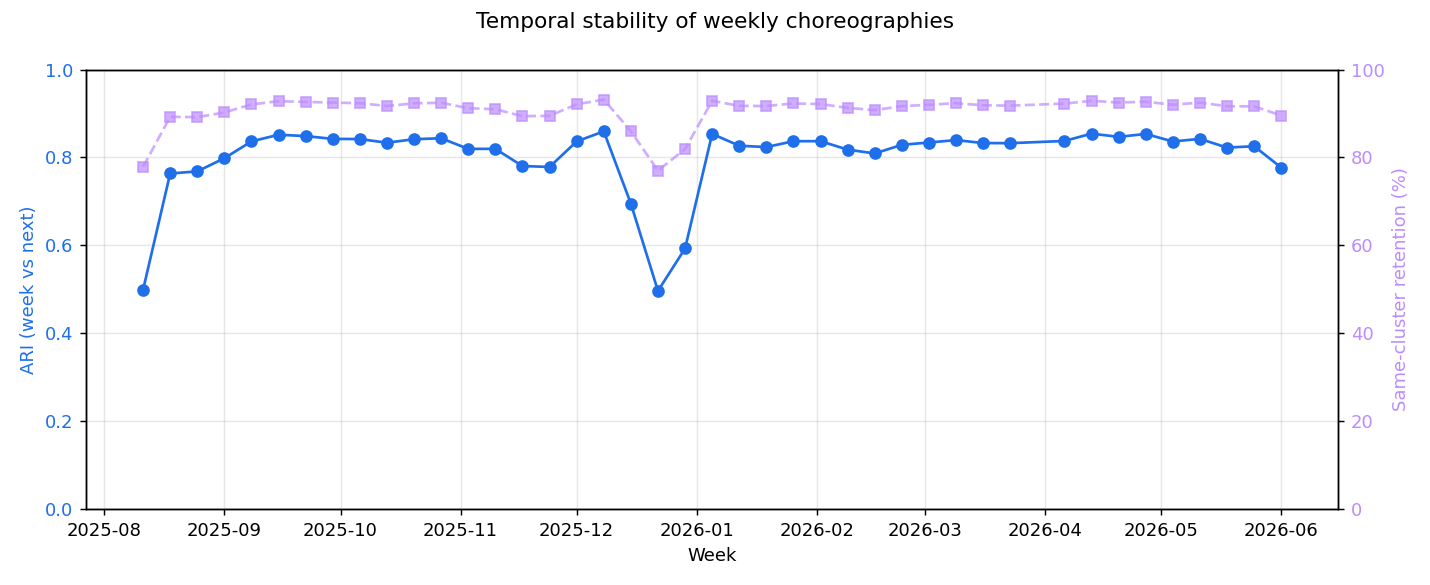
\includegraphics[width=0.85\textwidth]{figures/temporal_ari.png}
    \caption{Temporal stability of weekly choreographies, displaying week-over-week ARI (blue solid line) and same-cluster retention rates (purple dashed line).}
    \label{fig:temporal_ari}
\end{figure}

The transition matrix (Figure~\ref{fig:transition_matrix}) confirmed the "stickiness" (or inertia) along the main diagonal of each group, but with clear differences between them. The Steady Worker was the most stable, retaining 95.6\% of its members from one week to the next. The Balanced Engager showed solid retention at 91.9\%, and the Low Engagement profile kept 87.9\%. The Night Crammer proved the most volatile, retaining only 79.2\% of its students, with many shifting to other behavioral patterns in subsequent weeks. Notably, when students did leave the Night Crammer profile, they moved most often into the Low Engagement profile (around 9\% of transitions), suggesting a possible trajectory of disengagement over time.

\begin{figure}[H]
    \centering
    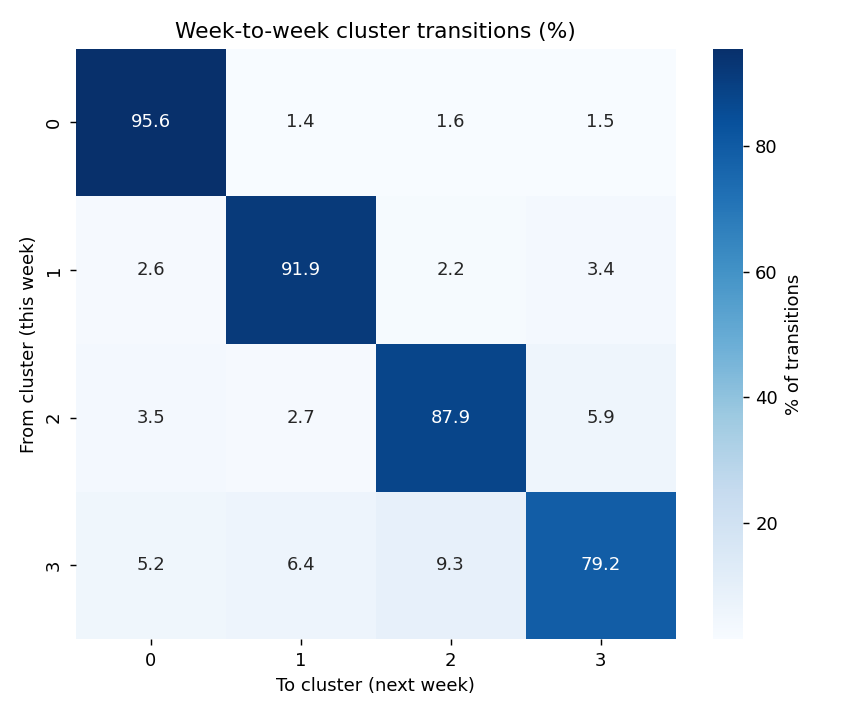
\includegraphics[width=0.50\textwidth]{figures/transition_matrix.png}
    \caption{Week-to-week cluster transition matrix (\%), highlighting the inertia along the main diagonal for each distinct behavioral profile.}
    \label{fig:transition_matrix}
\end{figure}

The cross-context stability analysis demonstrated that the discovered learning patterns are remarkably consistent and independent of geography or student age. The presence of the four profiles was nearly identical across all regions and grade levels, as illustrated in Figures~\ref{fig:dist_grade} and~\ref{fig:dist_state}. The variation (spread) between contexts stayed consistently below 3.5 percentage points, indicating that the profiles appear uniformly rather than reflecting a specific year's curriculum or a particular state's policies.

\begin{figure}[H]
    \centering
    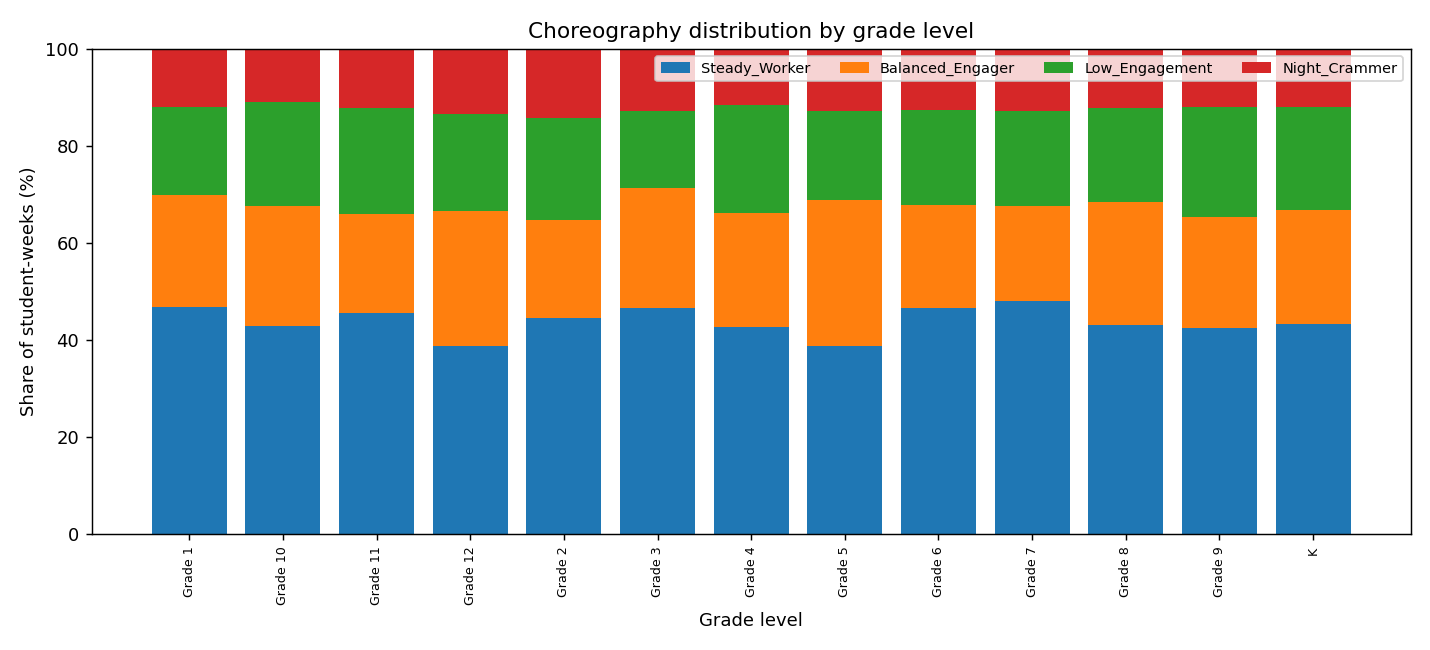
\includegraphics[width=0.9\textwidth]{figures/profile_by_grade.png}
    \caption{Choreography distribution by grade level, showing a highly consistent share of student-weeks across all K-12 grades.}
    \label{fig:dist_grade}
\end{figure}

\begin{figure}[H]
    \centering
    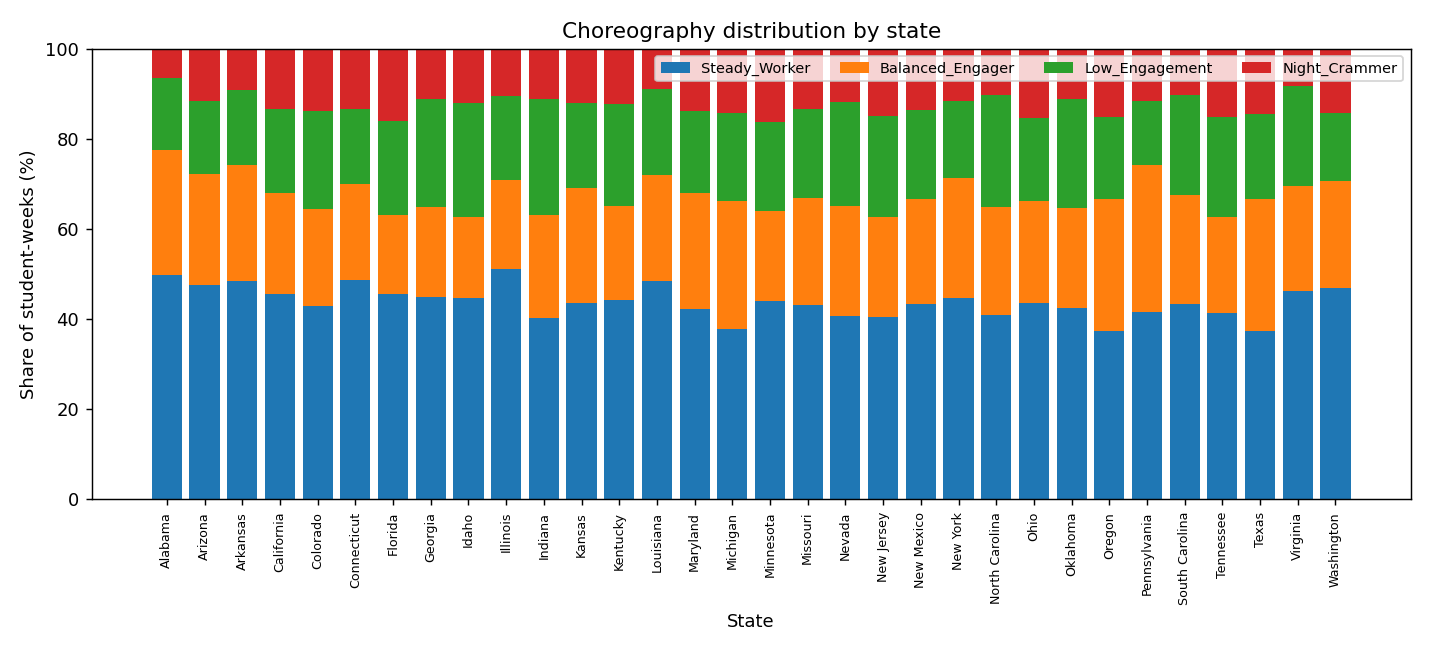
\includegraphics[width=0.9\textwidth]{figures/profile_by_state.png}
    \caption{Choreography distribution by state, demonstrating uniform profile presence across different geographical regions.}
    \label{fig:dist_state}
\end{figure}

Furthermore, when cosine similarity was used to compare whether the "shape" of platform behavior differed between younger students (elementary school, K-5) and older ones (secondary school, 6-12), the result was approximately 0.9999. This confirms mathematically that the behavioral signature of each profile remains essentially the same across schooling levels: the actions that define a Night Crammer in 3rd grade correspond to the exact same pattern of activity and timing in a 10th-grade student.

\section{RQ3: Association with Outcomes}
\label{sec:rq3-results}
% TODO: Present the outcomes-by-dominant-choreography summary table:
%   - Columns: n_students, avg_final_grade, avg_quiz, avg_completion, pass_rate.
%   - Order clusters by avg_final_grade descending.
%
% Report the ANOVA result:
%   - F-statistic, p-value, eta-squared effect size.
%   - State whether differences are statistically significant.
%
% Present the at-risk-stratified comparison:
%   - Mean Final_Grade for not-at-risk and at-risk students within each cluster.
%   - Note any cells with n = 0 (structural absence due to archetype-at-risk
%     correlation in the generator) and explain what this implies.
%   - Include grade_by_cluster.png and grade_by_cluster_atrisk.png.
The analysis revealed a clear hierarchy in both average grades and pass rates across the four profiles (see Figure~\ref{fig:final_grades}). At the top, with virtually identical and very positive results, were the Balanced Engager and the Steady Worker. The Balanced Engager led slightly, with an average grade of 74 and a pass rate of 82\%, followed closely by the Steady Worker, with an average of 73 and 81\% of its students passing. In an intermediate position, the Night Crammer recorded an average grade of 69 and a lower pass rate of 70\%. At the bottom was the Low Engagement profile: students with this dominant choreography reached an average grade of only 62 and a pass rate of 52\%, meaning barely more than half of this group passed.

\begin{figure}[H]
    \centering
    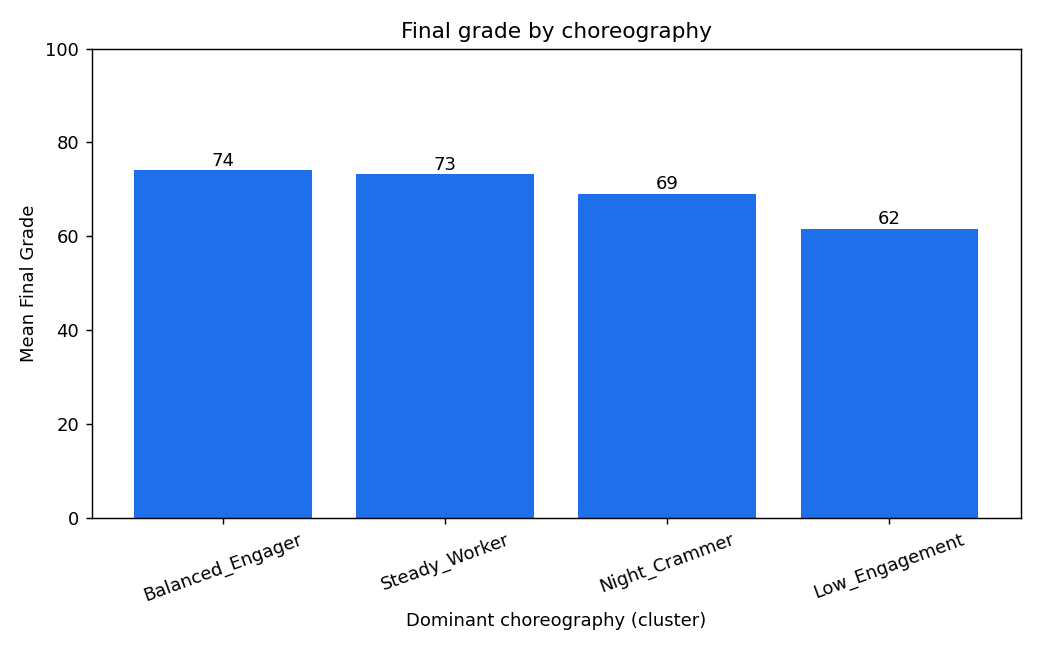
\includegraphics[width=0.85\textwidth]{figures/grade_by_cluster.png}
    \caption{Mean final grade by dominant choreography, illustrating the performance hierarchy among the four behavioral profiles.}
    \label{fig:final_grades}
\end{figure}

To assess the performance differences observed between the profiles, the ANOVA test offered two distinct perspectives, and it is essential to separate statistical significance from the actual magnitude of the effect. In terms of significance, the test returned a very high F-statistic (F~=~907) with a p-value below 0.001, indicating that the variation in average grades between the four groups is statistically significant rather than due to chance. On its own, however, significance can be misleading: in large samples the test is so sensitive that almost any minor fluctuation produces a very low p-value, which could lead to overvaluing irrelevant differences. The effect size addresses this. The eta-squared value ($\eta^2 \approx 0.35$) measures the practical weight of the result and shows that the difference is genuinely large, meaning the behavioral profile explains roughly 35\% of the total variance in students' final grades. Taken together, these metrics indicate not only that grade differences exist between the groups, but that they are substantial and strongly associated with how students engage with the platform.
    
Introducing the at-risk history into the analysis added an essential layer of honesty to the results, revealing two important points (as illustrated in Figure~\ref{fig:at_risk_control}). First, where a direct comparison was possible, at-risk status showed a negative effect of its own, independent of how the student studied. Within the same choreography, at-risk students consistently scored about 10 to 12 points lower than their non-flagged peers: in the Steady Worker group, the average fell from 73.9 to 63.3, and in the Night Crammer group, from 73.4 to 61.3. Second, this analysis runs into a serious limitation in the distribution of the data. The Balanced Engager profile contained almost no at-risk students, while the Low Engagement profile was composed almost entirely of them. This lack of overlapping students across groups means that choreography and initial risk status are strongly confounded by construction. As a result, the two effects cannot be fully disentangled: it is not possible to determine with full rigor whether a Low Engagement student's failure stems from their low-engagement routine itself, or whether it reflects the academic difficulties they already carried beforehand.

\begin{figure}[H]
    \centering
    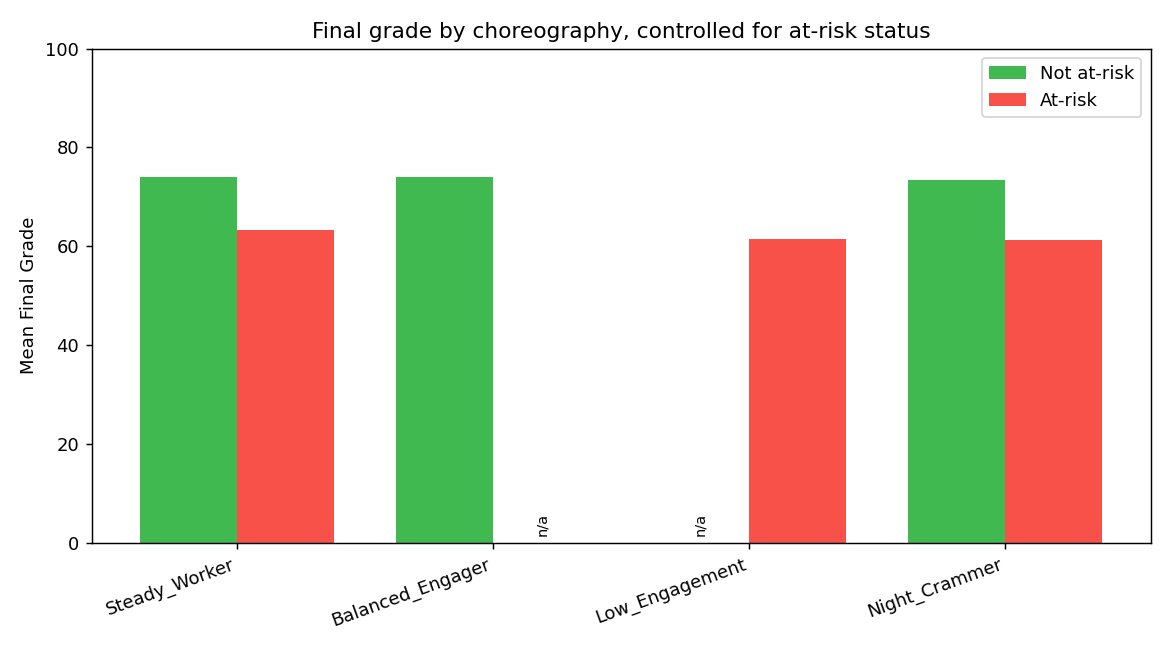
\includegraphics[width=0.85\textwidth]{figures/grade_by_cluster_atrisk.png}
    \caption{Mean final grade by choreography, controlled for at-risk status. Note the missing data (n/a) indicating the confounding between the Balanced Engager and Low Engagement profiles with baseline risk.}
    \label{fig:at_risk_control}
\end{figure}

\section{RQ4: Predictive Utility}
\label{sec:rq4-results}
% TODO: Present early prediction results for both time windows (first 4 weeks,
% first 8 weeks):
%   - Table with accuracy, F1, and ROC-AUC for baseline and experimental models
%     at each window.
%   - Report the AUC gain (experimental − baseline) at each window.
%   - Include rq4_comparison.png (AUC over time windows for both models).
%   - Discuss what the gain (or its magnitude) implies about how early the
%     choreography signal becomes detectable.
Looking at the results objectively, the baseline model sits consistently above the experimental model, as shown in Figure~\ref{fig:rq4_prediction}. The numbers confirm this clearly: at 4 weeks, the baseline reached an ROC-AUC of 0.825, while the experimental model (volume + choreography) fell slightly below at 0.824. At 8 weeks, the same pattern held, with the baseline at 0.838 and the experimental model at 0.833. The direct answer, therefore, is that the choreography did not improve the model's predictive performance. Adding the behavioral profile produced a negative AUC gain—in practice, the choreography added no predictive power over a simple count of interaction volume.

However, the RQ4 result carries a dual message, and the second part is highly positive. Early prediction of student success works and is reliable: in a setting with imbalanced classes, predicting the outcome as early as week 4 with an AUC around 0.83 is a strong and solid result. What this experiment ultimately indicates is a principle of parsimony. The early-warning signal works well from the start of the semester, but for strictly predictive purposes, knowing \textit{how much} a student works is sufficient, without needing to add complex information about \textit{how} they work.

\begin{figure}[H]
    \centering
    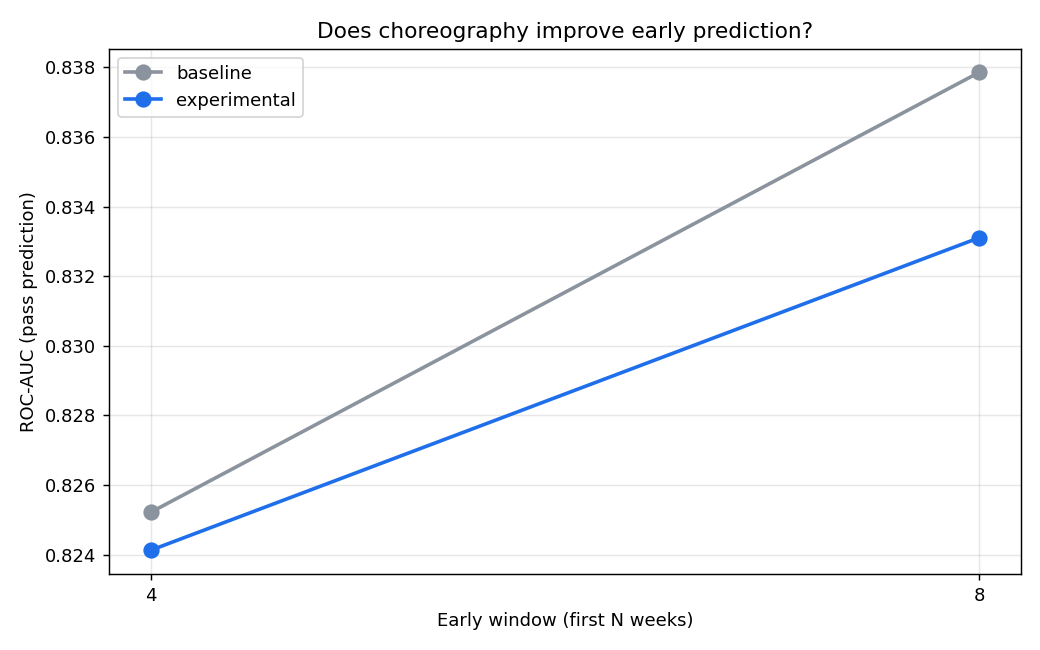
\includegraphics[width=0.85\textwidth]{figures/rq4_comparison.png}
    \caption{ROC-AUC comparison between the baseline model (volume only) and the experimental model (volume + choreography) at 4 and 8 weeks.}
    \label{fig:rq4_prediction}
\end{figure}

\section{RQ5: Actionability and Interpretation}
\label{sec:rq5-results}
% TODO: Present the feature importance results:
%   - Table of top features ranked by permutation importance, with their
%     Gini importance alongside for comparison.
%   - Direction-of-effect table: for the top 8 features, pass rate in the
%     bottom third vs top third, and the direction arrow.
%   - Note any discrepancy between Gini and permutation rankings (high-cardinality
%     features inflated in Gini).
%   - If SHAP was computed, present the top 8 features by mean |SHAP| and confirm
%     alignment with permutation importance.
%   - Include rq5_importance.png.
%   - Translate the top features into plain-language pedagogical implications
%     (e.g., "more Content_Study proportion → higher pass rate").
The Random Forest model (which achieved a solid ROC-AUC of 0.86) yields a clear message by separating behaviors into two groups: indicators of success and signals of risk, as illustrated in Figure~\ref{fig:feature_importance}. On the success side, active participation and engagement volume emerge as the main drivers of passing. The strongest signal overall is the number of sessions: a high session count raises the probability of success from 71\% to 98\%. Starting and submitting assignments rank at the top of importance, lifting pass rates from 74\% to 94--95\%, and joining synchronous sessions is associated with a marked rise from 80\% to 93\%. Consuming content, watching videos and studying course materials also proved strongly associated with passing.

\begin{figure}[H]
    \centering
    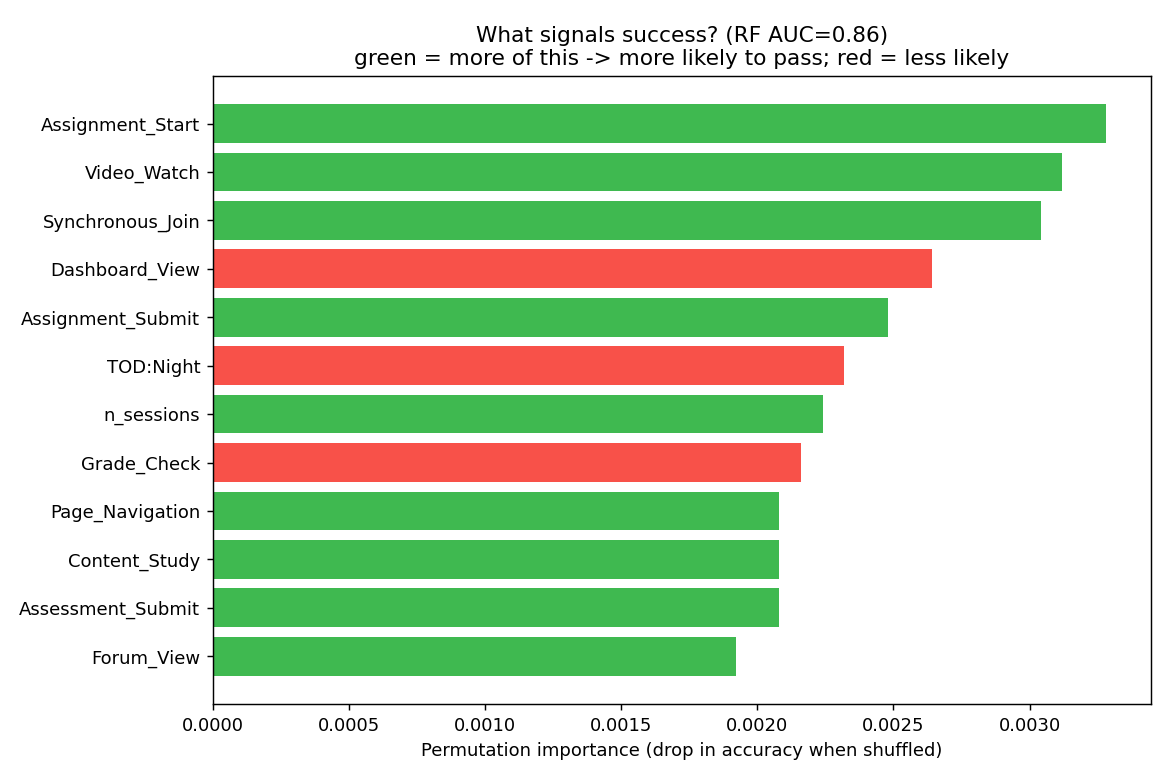
\includegraphics[width=0.85\textwidth]{figures/rq5_importance.png}
    \caption{Permutation feature importance (drop in accuracy when shuffled). Green bars indicate behaviors that signal a higher likelihood of passing, while red bars flag risk signals.}
    \label{fig:feature_importance}
\end{figure}

On the risk side, the model surfaces the most counter-intuitive finding of the analysis. Studying late at night is associated with a higher risk of failure. More strikingly, the model flags "unproductive navigation": excessive visits to the dashboard and repeated grade-checking as harmful, students whose activity is dominated by this kind of clicking see their pass rate fall from 95\% to 73\%. The key lesson is that merely being "online" is not the same as producing work. A student who appears active on a teacher's dashboard, but whose activity is dominated by refreshing the home page and repeatedly checking grades, may in fact be caught in a cycle of unproductive monitoring and at high risk of failing, signaling a need for intervention.

It should be noted that the model identifies statistical associations rather than causal relationships. Furthermore, the extreme sharpness of these behavioral signals partially reflects the underlying rules of the synthetic data generation process, a limitation that will be further addressed in the discussion.